\documentclass[12pt,floatfix,showpacs]{revtex4-1}

\usepackage{amssymb,amsmath,amsfonts}
\usepackage{graphicx}
\usepackage{subfig}

\newcommand{\eg}{\emph{e.g., }}
\newcommand{\ie}{\emph{i.e., }}
\newcommand{\etal}{\emph{et al.}}

% remove these for final publication 
\usepackage{color} 
\newcommand{\note}[1]{\textcolor{red}{#1}}
\newcommand{\gnote}[1]{\marginpar{\textcolor{red}{\scriptsize{#1}}}}

\graphicspath{{./graphics/}}

\begin{document}

\title{Eqtools: Modular, Extensible, Open-Source, Cross-Machine Python Tools for Working with Magnetic Equilibria}

\author{M. A. Chilenski}
\email[]{markchil@psfc.mit.edu}
\affiliation{MIT Plasma Science and Fusion Center}

\author{I. C. Faust}
\affiliation{MIT Plasma Science and Fusion Center}

\author{J. R. Walk}
\affiliation{MIT Plasma Science and Fusion Center}

\date{\today}

\begin{abstract}
 An introduction to the eqtools package, a modular, extensible, open-source toolkit in the Python programming language for handling magnetic equilibria from tokamaks, is presented.  The eqtools package provides a single interface for working with magnetic equilibrium data, both for handling derived-quantity data and mapping between coordinate systems in the flux grid, extensible to function with data from different experiments, data formats, and magnetic-reconstruction codes, replacing the static solutions currently used on tokamak experiments.  Moreover, the development of magnetic-equilibrium functionality in the Python language removes a substantial barrier to code migration and new development in Python, which presents a number of attractive advantages.  In this paper, we introduce the modular structure and design of the eqtools package and detail the workflow for usage and expansion to additional devices.  The implementation of a novel three-dimensional spline solution (in two spatial coordinates and in time) for improved timebase accuracy is also detailed.  Finally, Benchmarking for accuracy and speed against existing methods are detailed.
\end{abstract}
\gnote{other PACs numbers?}

\pacs{52.55.Fa}

\maketitle

%%%%%%%%%%%%%%%%%%%%%%%%%%%%%%%%%%%%%%%%%%%%%%%%%%%%%%%%%%%%

\section{Introduction}\label{sec:intro}

The basic computational tasks associated with magnetic-equilibrium reconstructions -- namely, the handling of derived quantities (\eg calculated plasma current, safety-factor profiles) and the mapping between real-space and flux coordinate systems for experimental data -- are universal among tokamak experiments.  Despite this commonality, experiments typically utilize in-house solutions developed for the particulars of that experiment's data storage and usage.  This ad-hoc development of base-level functionality inhibits the mobility of higher-level codes to other devices (as the code may require substantial modification to address the particulars of the new data storage design).  Moreover, such development is often quite static, such that the implementation is difficult to extend to new data formats (for example, to handle both a primary MDSplus-based data storage system \note{cite?} and the \emph{eqdsk} storage files produced directly by the EFIT reconstruction code \cite{Lao1985}), necessitating parallel workflows for functionally identical tasks depending on the data source.  Best design practices call for the vagaries of data source and storage implementation to be placed in the back end, presenting a consistent, straightforward interface common between machines and code implementations to the research scientist.

The new \emph{eqtools} package provides a modular, extensible, cross-machine toolkit developed in the Python programming language for handling magnetic-equilibrium data.  The \emph{eqtools} package provides a consistent \& straightforward interface to the researcher for both coordinate-mapping routines (which are historically handled in separate standalone routines) and derived-quantity data handling (which are often handled with manual hooks into data storage).  Moreover, \emph{eqtools} is constructed in a modular, object-oriented design, such that the package is easily extensible to handle data from different experiments and reconstruction codes, allowing the researcher a single unified interface for data from any machine or code.  The implementation of reconstructed-equilibrium handling in the Python language removes a substantial barrier to the adoption of Python as a day-to-day working language for tokamak research, which offers numerous advantages in ease of use, computational speed, user/developer base, and free \& open-source implementations compared to current common working languages for fusion research.\gnote{where to point to github?}

This paper details the design and implementation of the eqtools package, particularly the paradigm for extension to new machines (section \ref{sec:design}), describes the implementation of a trivariate spline method for improved coordinate-mapping accuracy in the time dimension (section \ref{sec:trispline}), and presents runtime and accuracy benchmarks against the current IDL implementation at Alcator C-Mod (section \ref{sec:benchmark}).

\section{Package Design and Use}\label{sec:design}

\begin{figure}[ht]
 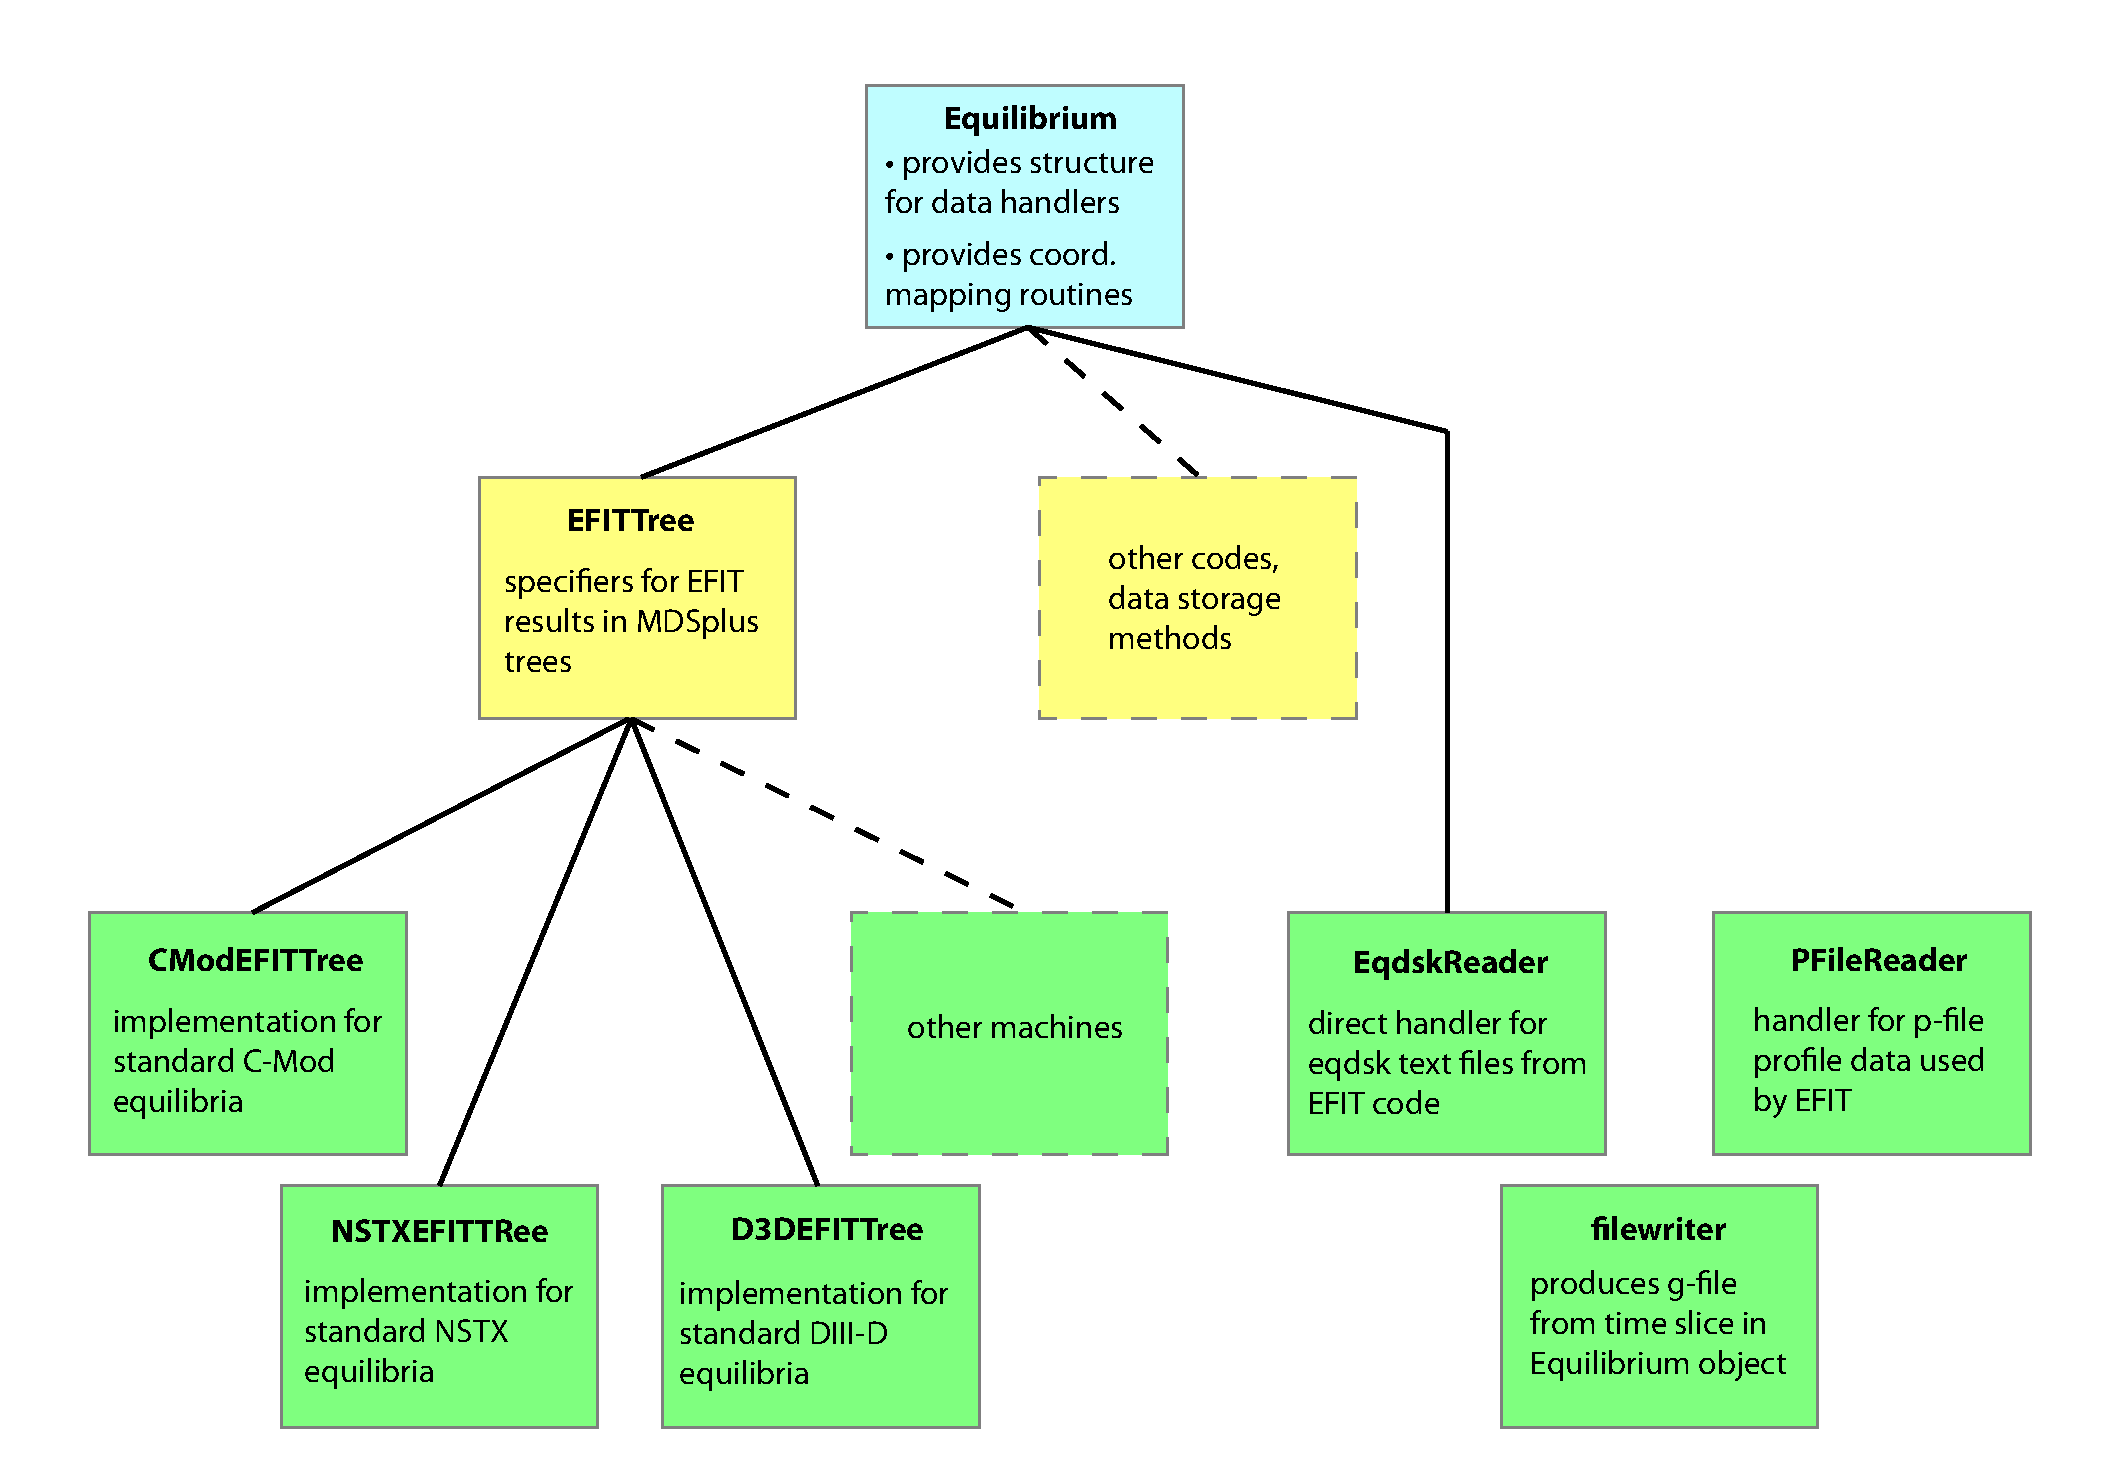
\includegraphics[width=\textwidth]{graphics/flowchart.pdf}
 \caption{}
 \label{fig:flowchart}
\end{figure}

\section{Tri-Spline Implementation}\label{sec:trispline}

\section{Benchmarking}\label{sec:benchmark}

\begin{figure}[ht]
 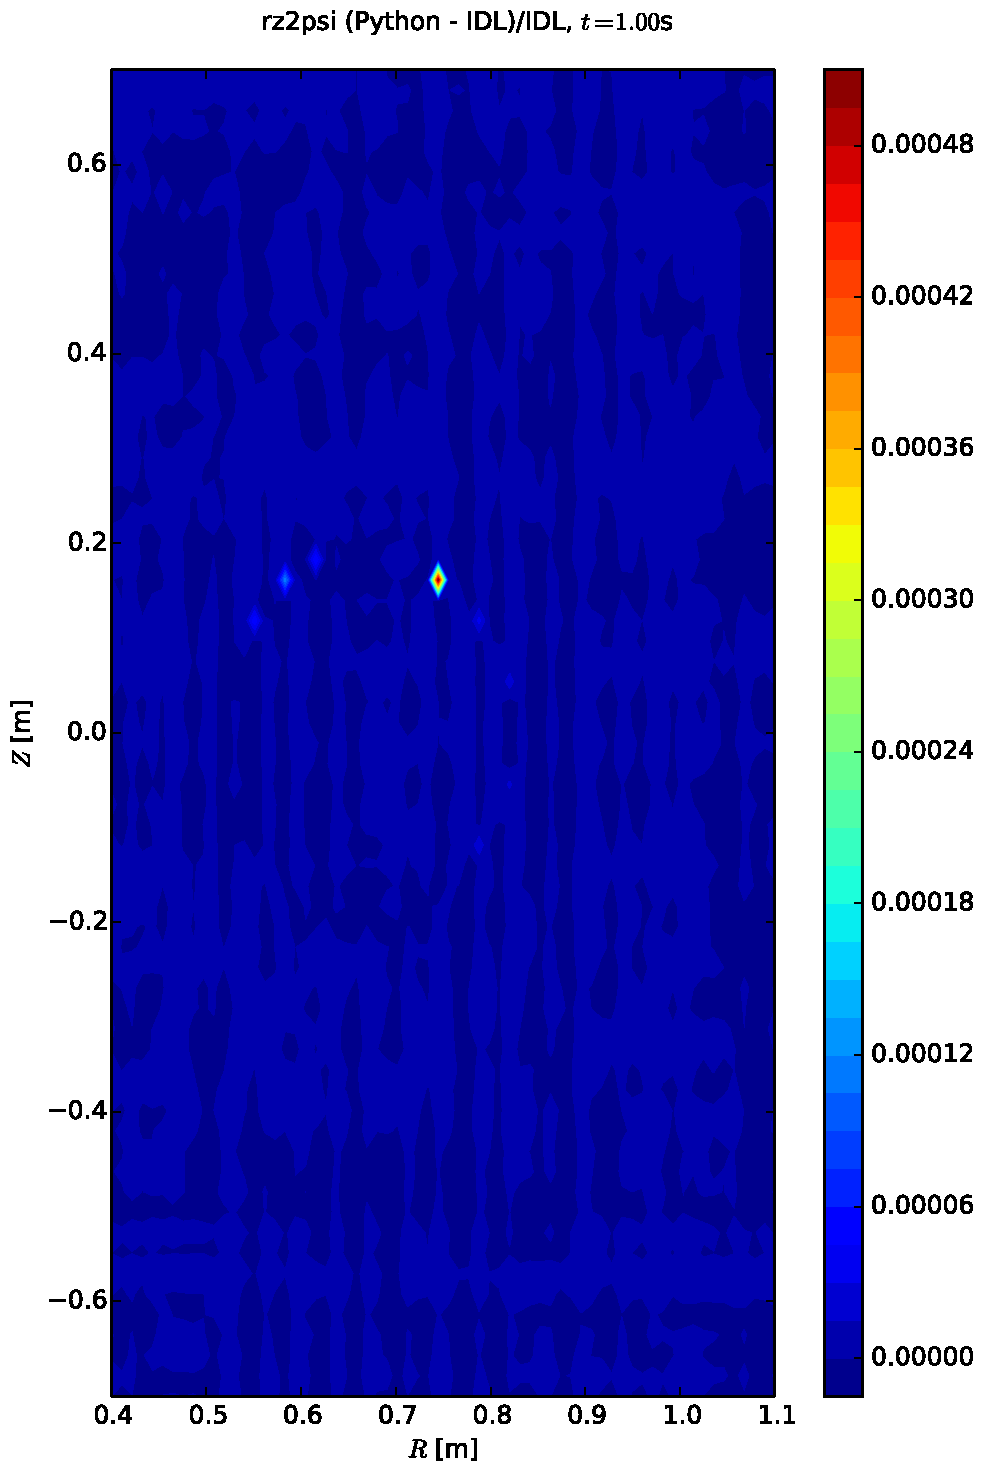
\includegraphics[width=13.65cm]{graphics/RZ2psi_rel_diff.pdf}
 \caption{Relative difference between calculations of a mapping between the RZ grid and poloidal flux for the \emph{eqtools} and the current IDL implementation of the mapping routine for an example Alcator C-Mod reconstructed equilibrium.  Relative differences of less than half a percent are typical.  \note{source of diff?  EFIT, spline error?}}
 \label{fig:rz2psi_diff}
\end{figure}

\section{Summary}\label{sec:summary}

%%%%%%%%%%%%%%%%%%%%%%%%%%%%%%%%%%%%%%%%%%%%%%%%%%%%%%%%%%%%

\begin{acknowledgements}
 acknowledgements go here.
\end{acknowledgements}

\bibliographystyle{aipnum4-1}
\bibliography{eqtools_paper}

\end{document}